\documentclass[12pt,letterpaper]{article}
\usepackage{setspace,float,csquotes}
\usepackage[pdftex]{graphicx}
\setlength{\textwidth}{6.5in}
\setlength{\oddsidemargin}{0in}
\setlength{\textheight}{9in}
\setlength{\topmargin}{-.25in}
\doublespacing
\title{Vehicle Database}
\author{Warvin Hassan}
\begin{document}
	\maketitle
	\pagebreak
	\textbf{Introduction:}
	Climate change is real, and one of the biggest contributors to that are vehicles. For this paper, it is assumed that the reader has knowledge of databases equivalent to an introductory database student. This paper serves as a follow-up to the final project presentation on my vehicle database, done in class, and effectively describes the process of how I created and used a database to illuminate the threat of CO2 emissions from vehicles. The goal is to identify the main culprit of these emissions using mock data, focusing on the specific types of vehicles and their associated emissions. The database schema was designed to capture relevant details while ensuring scalability for future data integration. The relationships between the various entities, such as person, vehicle, and engine, were modeled using normalized tables. This structure allows for efficient data storage and retrieval, while minimizing redundancy. The mock data used in this paper includes variables such as vehicle make, model, engine type, and emissions, all of which contribute to understanding the environmental footprint of different vehicles. By analyzing these data points, we can identify which vehicle types and engine configurations are the most significant contributors to CO2 emissions. 
	
	\textbf{Implementation:}
	For the data collection phase, I leveraged ChatGPT to generate mock data based on common vehicle categories with the following prompt:
	\begin{displayquote}
		“I want 100 entries of raw data generated in the form of a csv file that mocks real data from 2015 until now. I want the columns to be based off of this schema: Owner information, such as fullname, and address(street1,street2optional,city,state,postal) Vehicle information such as year, make, model, plateID and Statecode, engine type and the emissions produced based off of miles driven (for electric I want emissions produced from production fossil fuels since they don't really produce anything on their own). As for the vehicle types (electric, hybrid, and gas) I want data on the battery capacity and range of electric types, battery capacity and fuel efficiency of hybrids and fuel efficiency of gas types. Also, some optional data meaning they don't all have to have data on these columns: registrationDate, salesAmount, salesDate.” 
	\end{displayquote}
	Using the AI’s ability to simulate data from a range of automotive sources, I created a diverse dataset that includes vehicle makes, models, engine types, fuel efficiency ratings, and annual CO2 emissions estimates. This mock data aimed to represent various vehicle types, such as gas, electric vehicles, and hybrids, ensuring a wide coverage for the analysis. While the data generated is not representative of real-world figures, it was more so designed to almost accurately reflect the type of information typically found in publicly available automotive databases and governmental reports on emissions. The mock data provided a foundation for building out the database structure and allowed for meaningful queries and analysis of the relationship between vehicle characteristics and emissions outputs. For first normal form, I ensured that all attributes in the database contained atomic values, meaning each field only holds a single value. For example, the vehicle table contains distinct columns for make, model, and year, avoiding multiple values in a single column. For second normal form, I ensured that all non-key attributes in the database were fully functionally dependent on the primary key. For instance, the engine table stores CO2 emissions data that depends directly on the engineID.
	
	\textbf{Results:}
	This database was queried to generate insights into which vehicle types (electric, hybrid, gas) are most responsible for CO2 emissions. The main objective of this query was to identify vehicles with above-average CO2 emissions, in order to analyze the types of vehicles and engines contributing most to the environmental impact. The query selects relevant vehicle details, including the make, model, state, engine type, and annual CO2 emissions. It joins several tables—vehicle, engine, personvehicle, person, and address—to retrieve the necessary data and applies a sub-query that filters for vehicles whose emissions exceed the average emissions for all engine types. More specially, the columns make and model provide the vehicle's make and model, helping identify specific types of vehicles contributing to high emissions. State shows the residence for the vehicle owner, offering geographical context. engine\_type specifies the engine type for each vehicle (e.g., gas, hybrid, electric), which plays a critical role in determining which vehicle type is contributing to high emissions. Finally, annual\_CO2\_kg presents the annual CO2 emissions in kilograms, allowing for direct comparison across vehicles. The query returns a list of vehicles that have annual CO2 emissions higher than the average emissions for their respective engine types. The results are sorted in descending order of emissions, allowing for a clear view of which vehicles contribute most to CO2 output. The results clearly show that traditional gasoline-powered vehicles such as the Toyota RAV4 and Toyota Prius emit the most CO2 compared to their electric and hybrid counterparts, which produce significantly lower emissions. 
	\pagebreak
	\begin{table}[ht]
		\caption{\label{que}}  
		\begin{center}
			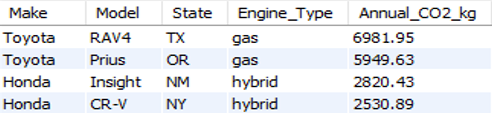
\includegraphics[width=\textwidth]{table.png}
		\end{center}
	{The resulted table of 4 rows to answer my question using the query in figure \ref{q}. Based off of the data in this table Toyota is the main contributor to annual CO2.}
	\end{table}
	\pagebreak
	\begin{figure}[ht]  
		\begin{center}
			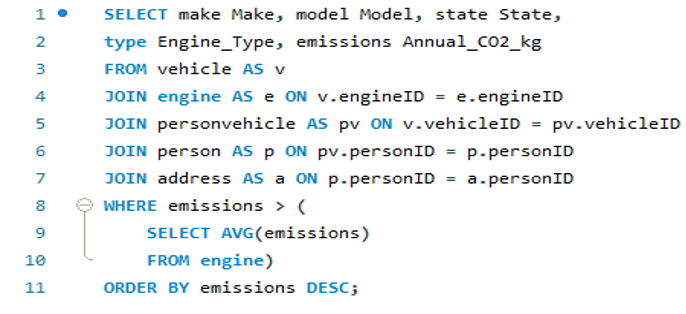
\includegraphics[width=\textwidth]{q.jpg}
		\end{center}
		\caption{\label{q} The query to table 1 that joins respective tables and compares emissions to average emissions.}
	\end{figure}
	\pagebreak
	\begin{figure}[ht]  
		\begin{center}
			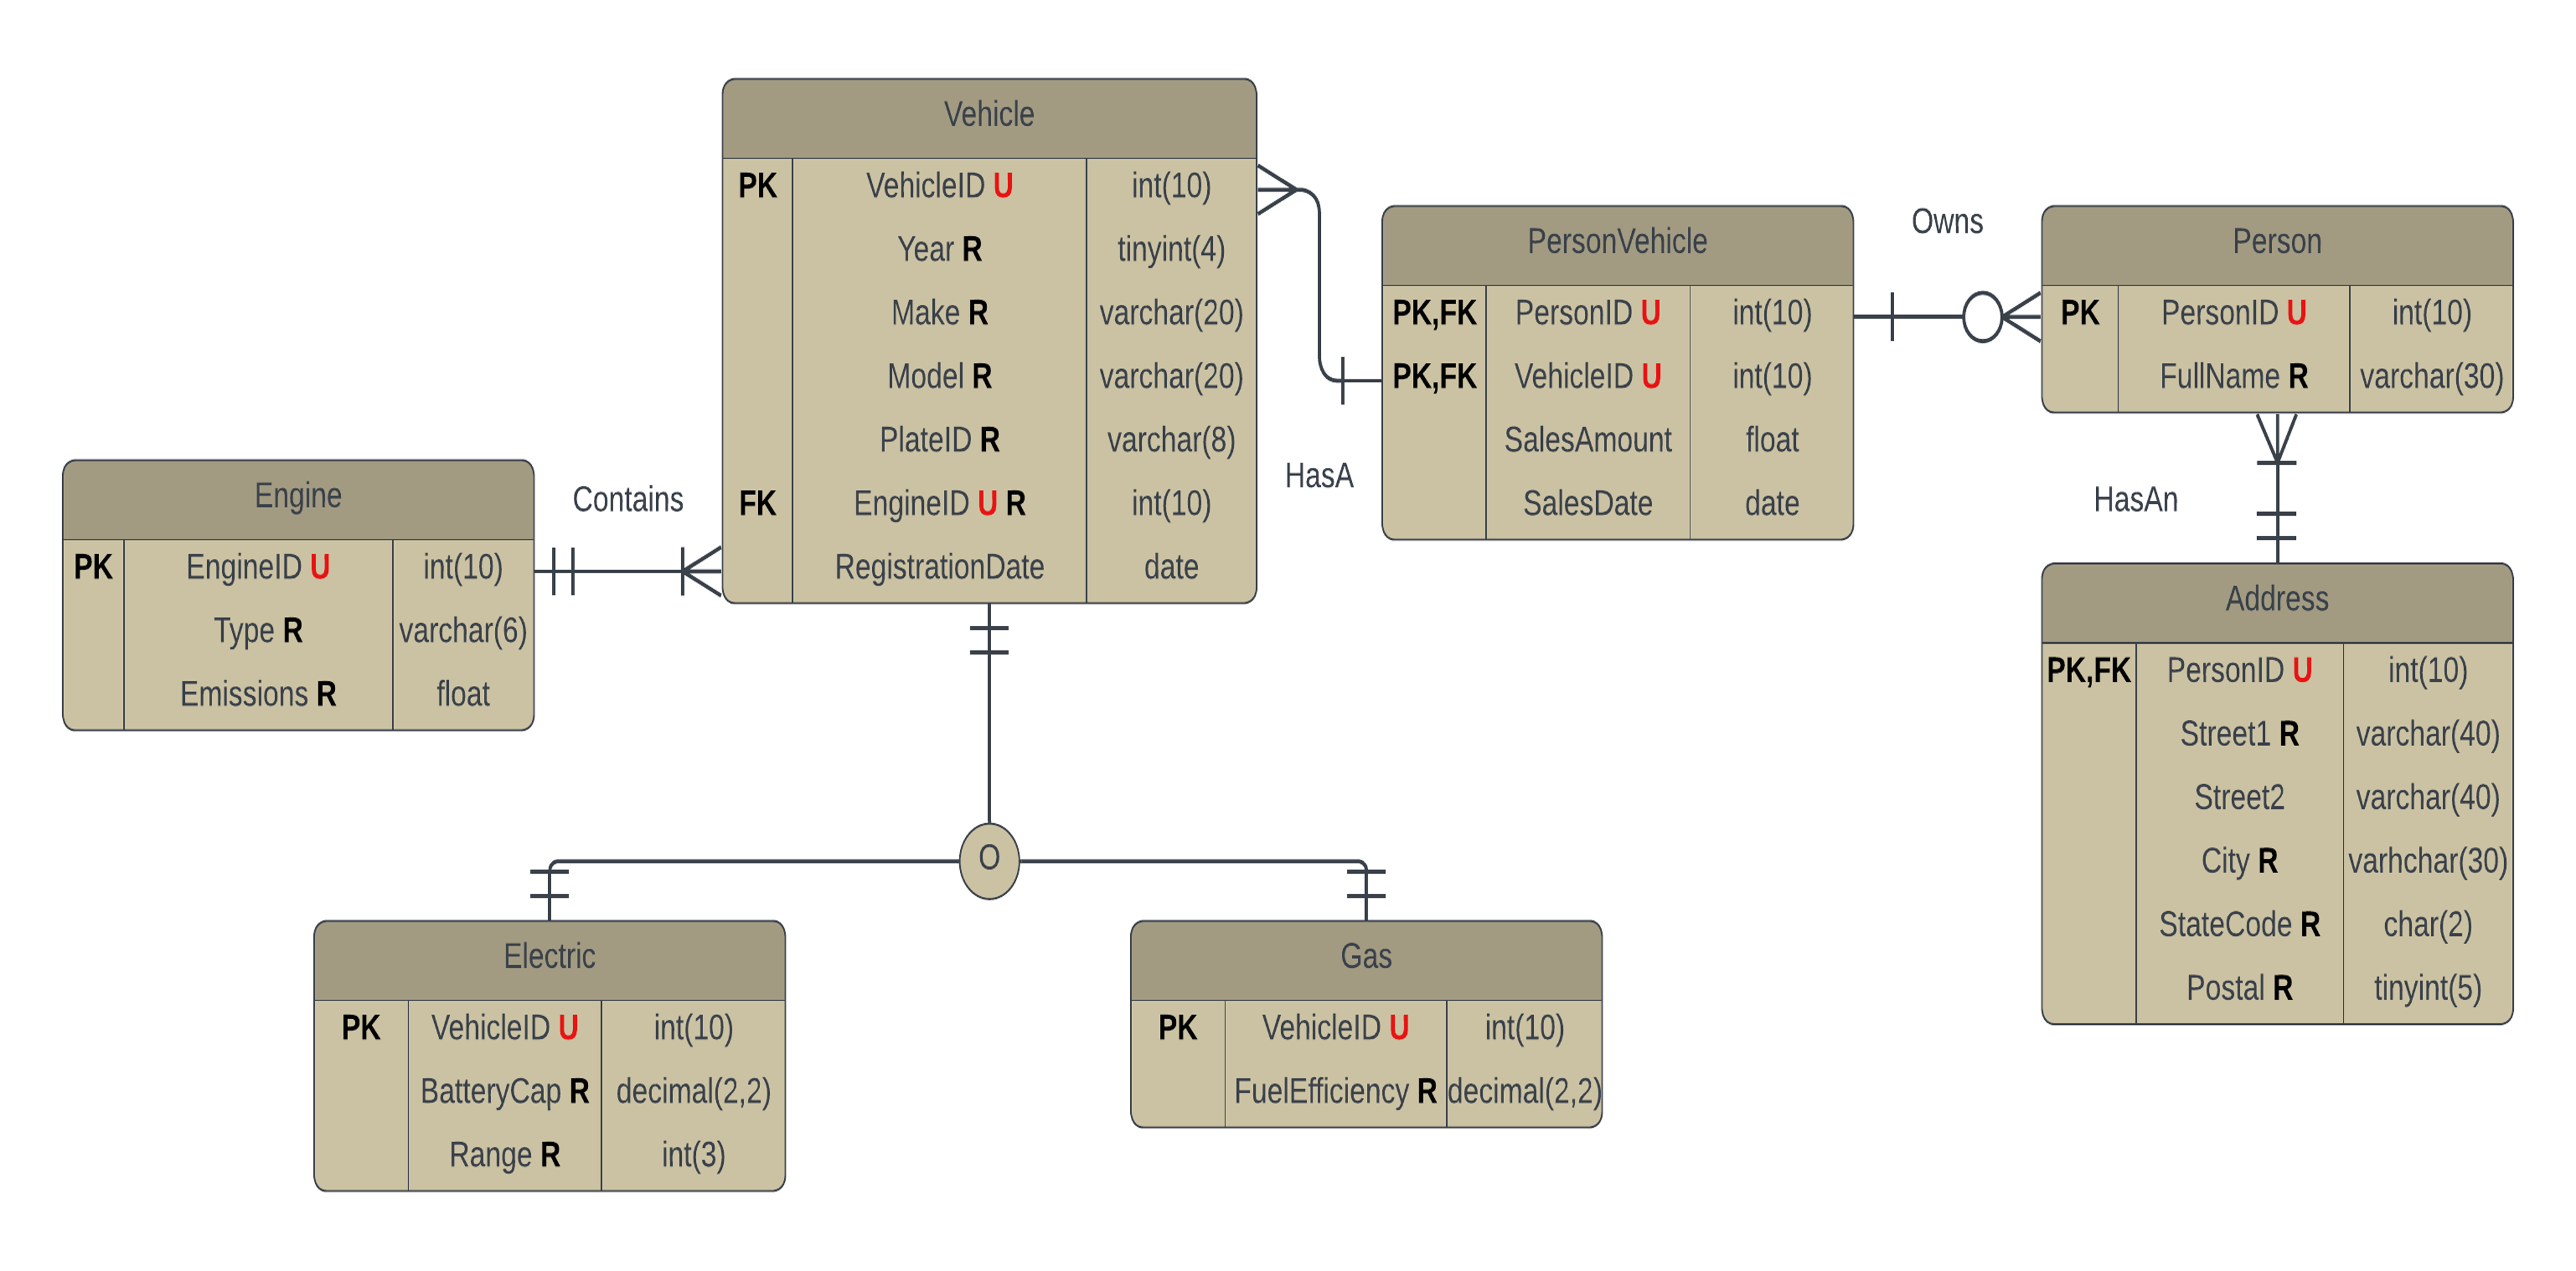
\includegraphics[width=\textwidth]{tdia.jpg}
		\end{center}
		\caption{\label{table} The vehicle table diagram used for the creation of my schema.}
	\end{figure}
	\pagebreak
	\begin{figure}[ht]  
		\begin{center}
			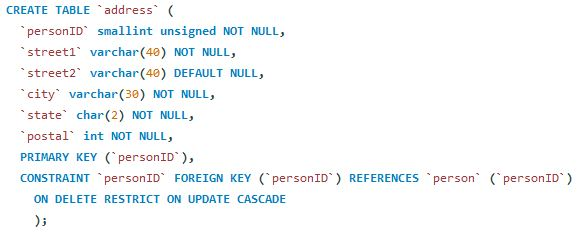
\includegraphics[width=\textwidth]{address.jpg}
		\end{center}
		\caption{\label{address} Query used to create address table.}
	\end{figure}
	\pagebreak
	\begin{figure}[ht]  
		\begin{center}
			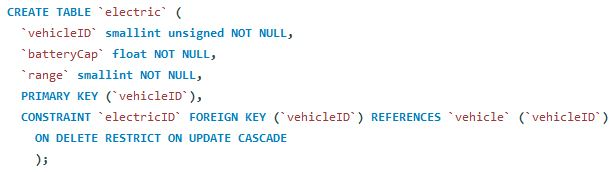
\includegraphics[width=\textwidth]{electric.jpg}
		\end{center}
		\caption{\label{electric} Query used to create electric subtable.}
	\end{figure}
	\pagebreak
	\begin{figure}[ht]  
		\begin{center}
			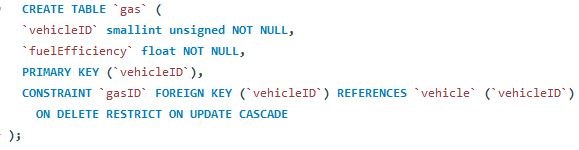
\includegraphics[width=\textwidth]{gas.jpg}
		\end{center}
		\caption{\label{gas} Query used to create gas subtable.}
	\end{figure}
	\pagebreak
	\begin{figure}[ht]  
		\begin{center}
			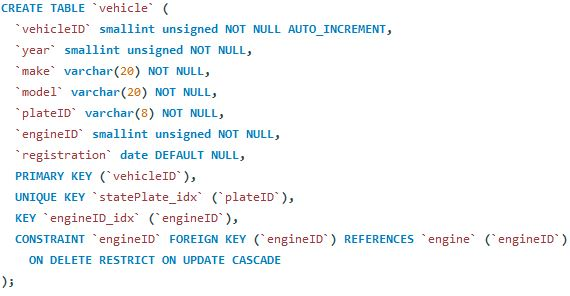
\includegraphics[width=\textwidth]{vehicle.jpg}
		\end{center}
		\caption{\label{vehicle} Query used to create vehicle table.}
	\end{figure}
	\pagebreak
	\begin{figure}[ht]  
		\begin{center}
			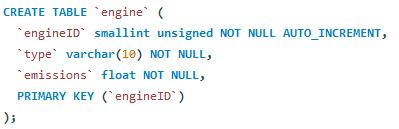
\includegraphics[width=\textwidth]{engine.jpg}
		\end{center}
		\caption{\label{engine} Query used to create engine table.}
	\end{figure}
	\pagebreak
	\begin{figure}[ht]  
		\begin{center}
			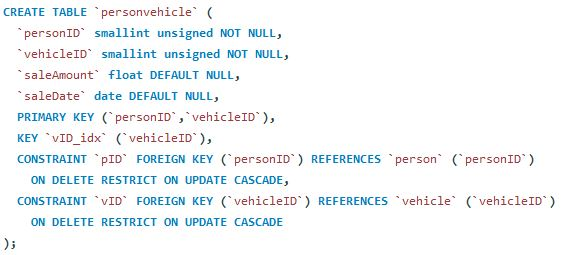
\includegraphics[width=\textwidth]{personvehicle.jpg}
		\end{center}
		\caption{\label{personvehicle} Query used to create personvehicle table.}
	\end{figure}
	\pagebreak
	\begin{figure}[ht]  
		\begin{center}
			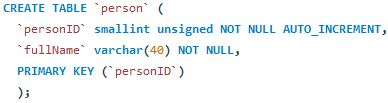
\includegraphics[width=\textwidth]{person.jpg}
		\end{center}
		\caption{\label{person} Query used to create person table.}
	\end{figure}
\end{document}